\documentclass[letter,10pt]{article}
\usepackage[letterpaper, lmargin=.5in, rmargin=.5in]{geometry}
\usepackage[utf8]{inputenc}
\usepackage{verbatim}
\usepackage{color}
\usepackage[]{amsmath}
\usepackage{mathtools}
\usepackage{pdfpages}
\usepackage{enumitem}
\usepackage{listings}
\usepackage{amssymb}
\usepackage{amsfonts}
\usepackage{graphicx}
\usepackage{subfig}
% \usepackage{pstool}
\usepackage{algorithm}
\usepackage{array}
\usepackage{tikz}
\usetikzlibrary{matrix}
\usepackage[binary-units]{siunitx}
\usepackage[backref=page,
            pageanchor=true,
            plainpages=false,
            pdfpagelabels,
            bookmarks,
            bookmarksnumbered,
            linkbordercolor={1 0.5 0.5},
            citebordercolor={0 0.5 0},
]{hyperref}

\usepackage{array,mathtools}
\newcommand*{\carry}[1][1]{\overset{#1}}
\newcolumntype{B}[1]{r*{#1}{@{\,}r}}

\newcommand{\eg}{\textit{e.g.},~}
\newcommand{\etc}{\textit{etc.}}
\let\eqref\undefined

\newcommand{\figref}[1]{Figure~\ref{fig:#1}}
\newcommand{\algoref}[1]{Algorithm~\ref{algo:#1}}
\newcommand{\secref}[1]{Section~\ref{sec:#1}}
\newcommand{\tabref}[1]{Table~\ref{tab:#1}}
\newcommand{\eqref}[1]{Equation~\ref{eq:#1}}
\newcommand{\figlabel}[1]{\label{fig:#1}}
\newcommand{\algolabel}[1]{\label{algo:#1}}
\newcommand{\seclabel}[1]{\label{sec:#1}}
\newcommand{\tablabel}[1]{\label{tab:#1}}
\newcommand{\eqlabel}[1]{\label{eq:#1}}

\DeclarePairedDelimiter\abs{\lvert}{\rvert}%
\DeclarePairedDelimiter\norm{\lVert}{\rVert}%


% Title Page
\title{CMPSCI 453\\HW7, Homework Problem Set 3}
\author{Tony Gao}

\begin{document}
\maketitle

%\begin{abstract}
%\end{abstract}

\section{Problem 1}

\begin{align}
01011011 + 01110010 = 
\begin{array}{B3}
 0 & \carry 0\carry 1 \carry 0 1 &  1 \carry 0 11 \\
{} + 0 &                             0111 &               0010 \\ \hline
0 &                             1100 &                      1101 \\
\end{array} \\
 +01100100 =
\begin{array}{B3}
\carry 0 & \carry 1 1 0 \carry 0&  \carry 1 1 0 1 \\
{} + 0 &                             0110 &               0100 \\ \hline
1 &                             0011 &                      0001 \\
\end{array} \\
\text{With wraparound} = 00110010 \\ 
\text{1's Complement} = 11001101
\end{align}

\begin{enumerate}
\item The receiver detects error with the 1's complement checksum by adding with wraparound all three 8-bit bytes, and then the checksum. If the sum is 0xFF, there are no errors. 

\item A 1-bit error cannot possibly go undetected. The error bit would result in the three 8-bit bytes adding to a different sum, such that adding the checksum would result in sum $\neq$ 0xFF. 

\item A 2-bit error could possibly go undetected. If one bit at the same significance index in two of the 8-bit words are flipped, the sum of the three words would still be the same, resulting in the same sum. For example, if the first two words were 01011010 + 01110011 instead of 01011011 + 01110010 (LSB flipped), the sum is clearly still the same. If a 2-bit error in the same 8-bit word occurred, then the error would be detected.
\end{enumerate}

\section{Problem 2}
\textbf{Deadlock condition:}
\begin{enumerate}
	\item Sender sends packet 0, transitions from state (Wait for call 0 from above) to (Wait for ACK or NAK 0)
	\item Receiver never receives packet 0, it is lost by the Sender's underlying Network/Link/Physical layer.
	\item Sender is waiting for ACK or NAK 0.
	\item Receiver is waiting for packet 0. Deadlock.
\end{enumerate}

\section{Problem 3}

\begin{enumerate}
	\item For infrequent data transfer: A protocol that uses ACK is preferable so packets that never make it to the receiver can be guaranteed to be resent in a short period of time. For example, given a packet n sent by A to B and is lost, B does not know that packet n is lost until it receives packet n+1 out of order, at which point it can send a NAK, but a long time may already have elapsed due to infrequent data transfer. ACK is clearly better here, since when A does not receive an ack for packet n within some time, A can infer a NAK and retransmit packet n.
	
	\item For high volume data transfer over a low-loss channel, a nak-only protocol is preferable. Because data is arriving at a high rate to the receiver, the amount of time to send a NAK for a lost packet becomes very small. There is a significant reduction in packets sent from receiver to sender in the NAK-only protocol versus the ACK-only protocol.
\end{enumerate}

\section{Problem 4}

\begin{center}
\noindent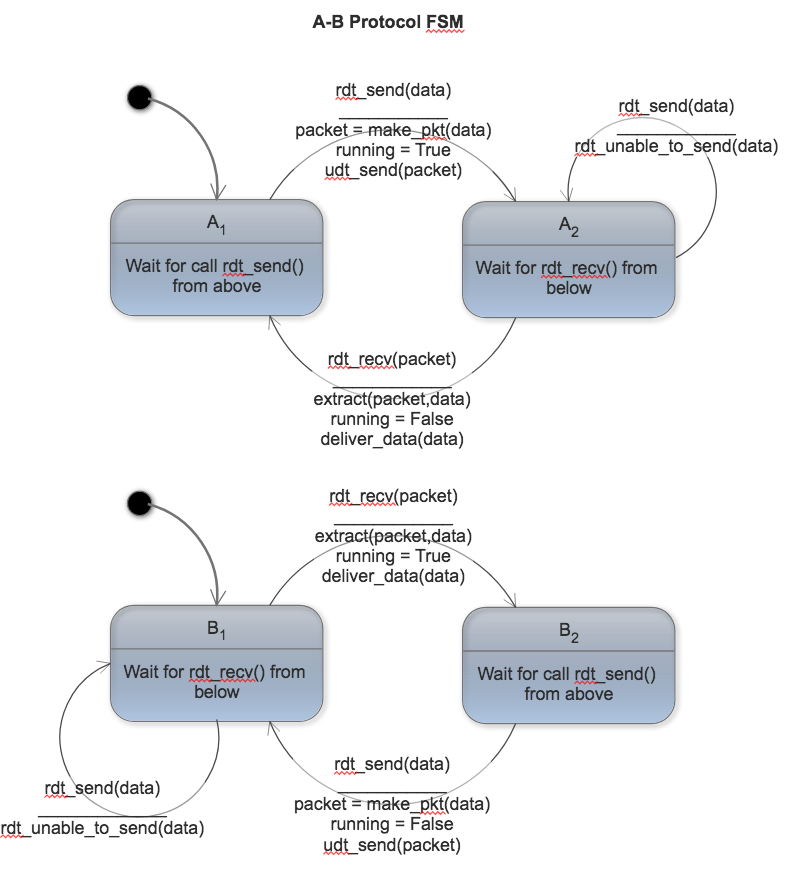
\includegraphics[height=.9\textheight,width=.9\textwidth]{./figures/abfsm}
\end{center}

\section{Problem 5}

\begin{enumerate}[label=\alph*)]
	\item Since the sequence number of the first segment is 147, and there are 80 bytes, the sequence number of the second segment would be $147 + 80 = 227$. The source port is 304. The destination port is 80.
	
	\item The acknowledgment number of the first byte is 227, which is the sequence number of the next byte expected from A. The source port number is 80, the destination port number is 304.

	\item  The ACK number for the first segment would be $147 + 80 + 40 = 267$. When the second segment arrives, B would send (ACK, 147) since 147 was the next expected sequence number. The second segment would be buffered. When the first segment arrives, B would send (ACK, 267) since both segments arrived. Finally, the transport layer of B will deliver these in order packets to the application layer.
	
	\item The first timeout expires, the ack for segment 2 is received after the first timeout expires. Since ack(267) $>$ SendBase(147), SendBase is set to 267. There are no more not-yet-acked segments, so the timer is stopped. When the first timeout expires, the sender has not yet received a cumulative ack that includes sequence 147, so sender retransmits 147, sets the second timeout, receives ack 267, and ignores it because ack(267) $\leq$ SendBase, so no action is taken by the sender state machine.
		\begin{center}
			\noindent 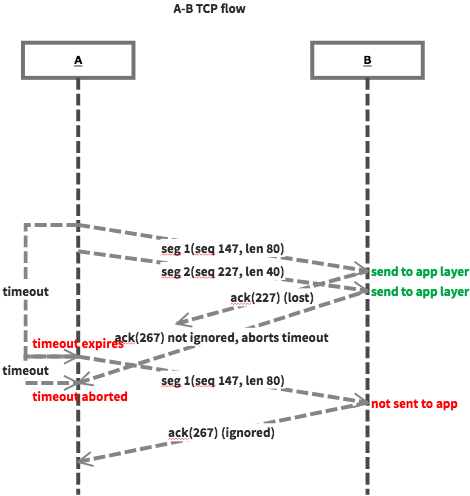
\includegraphics[height=.6\textheight]{./figures/5d}
		\end{center}		
\end{enumerate}

\section{Problem 6}

\begin{enumerate}[label=\alph*.]
	\item ~
	\begin{table} [h]
		\centering
		\begin{tabular}{|l|c|c|c|c|}
			\hline
			t & sender state   & receiver state        & packet type sent & seq \# or ACK \# sent \\ \hline
			0 & Wait for ACK 0 & Wait for 0 from below & data             & 0                     \\ \hline
			1 & Wait for ACK 0 & Wait for 1 from below & ack              & 0                     \\ \hline
			2 & Wait for ACK 0 & Wait for 1 from below & data             & 0                     \\ \hline
			3 & Wait for ACK 0 & Wait for 1 from below & ack              & 0                     \\ \hline
			4 & Wait for ACK 1 & Wait for 1 from below & data             & 1                     \\ \hline
			5 & Wait for ACK 1 & Wait for 0 from below & ack              & 1                     \\ \hline
			6 & Wait for ACK 0 & Wait for 0 from below & data             & 0                     \\ \hline
		\end{tabular}
	\end{table}

	\item The payload is delivered 2 times. Once for packet 1 (seq 0) and once for packet 3(seq 1). Packet 2 is received while receiver is in state (Wait for 1 from below) so it is not delivered. Data is passed up at t=1, t=5.
	
\end{enumerate}

\section{Problem 7}

\begin{align}
\alpha &= 0.125, \beta = 0.25 \\
EstimatedRTT &= (1 - \alpha) \cdot EstimatedRTT + \alpha \cdot SampleRTT \\
DevRTT &= (1 - \beta) \cdot DevRTT + \beta \cdot \abs*{SampleRTT - EstimatedRTT} \\
TimeoutInterval &= EstimatedRTT + 4 \cdot DevRTT \\
~
EstimatedRTT_0 &= 360ms\\
DevRTT_0 &= 21ms \\
~
SampleRTT_1 &= 270ms \\
DevRTT_1 &= (1 - .25) \cdot 21ms + .25 \cdot \abs*{270ms - 360ms} \\
&= 38.25ms \\
EstimatedRTT_1 &= (1 - 0.125) \cdot 360ms + 0.125 \cdot 270ms \\
&= 348.75ms \\
TimeoutInterval_1 &= 348.75ms + 4 \cdot 38.25ms  = 501.75ms\\
~
SampleRTT_2 &= 320ms \\
DevRTT_2 &= (1 - .25) \cdot 38.25ms + .25 \cdot \abs*{320ms - 348.75ms} \\
&=  35.875ms \\
EstimatedRTT_2 &= .875 \cdot 348.75ms + .125 \cdot 320ms \\
&= 345.15625ms \\
TimeoutInterval_2 &= 345.15625ms + 4 \cdot 35.875ms = 488.65625ms\\
~
SampleRTT_3 &= 250ms \\
DevRTT_3 &= (1 - .25) \cdot 35.875ms + .25 \cdot \abs*{250ms - 345.15625ms} \\
&= 50.6953125ms \\
EstimatedRTT_3 &= .875 \cdot 345.15625ms + .125 \cdot 250ms \\
&= 333.26171875ms \\
TimeoutInterval_3 &= 333.26171875ms + 4 \cdot 50.6953125ms = 536.042969ms 
\end{align}

\section{Problem 8}
The largest allowable sender window is of size $N \leq \frac{k}{2}$. This is the largest window that will guarantee that any resent packets as a result of dropped acks are definitely packets that were originally sent before the receive\_base pointer. If the window was larger, it is possible for the sender and receiver windows to desynchronize in both SR and GBN such that the receiver will believe retransmissions to be new packets. 

With a GBN sequence space of 2 and window size 2: if sender sends packets 0,1 back to back, and receiver acks 0,1 but both acks are lost, the sender window will be [0,1],0,1 and the receiver window will be 0,1,[0,1]. The sender would then retransmit 0 and 1 after timeout on 0 expires. Receiver will receive 0,1, deliver duplicate data upstream since it arrives in order and within the receiver window, and respond with ack. This moves sender window to 0,1,[0,1] and receiver window to 0,1,0,1,[0,1]. This delivers the same packets (0,1) twice upstream on the receiver side.

With a SR sequence space of 4 with window size 3 : if sender sends packets 0,1,2 back to back, and the receiver acks [0,1,2] but all acks are dropped, the sender window will still be at [0,1,2], but the receiver window will have progressed to [3,0,1]. The sender ack timeouts on 0,1,2 would tick retransmitting packets [0,1,2]. The receiver will receive packets 0 and 1 and believe that they are new packets since they lie within the current receiver window.  The receiver will discard packet 2. The receiver will ack packets [0,1,2] leading to sender sending packet 3, causing the receiver to deliver [3,0,1], of which only [3] is an actual new packet. \\

With a window size of 2, this problem is avoided. Sender sends [0,1]. Receiver ack [0,1] is dropped. Receiver window moves to [2,3]. Sender retransmits [0,1]. Receiver acks [0,1], discards retransmitted packets since $0,1 \leq SendBase - 1$. Sender window moves to [2,3]. Sender sends [2,3]. Receiver acks [2,3], windows are synchronized.

\section{Problem 9}
\begin{figure}[h!]
\begin{center}
	\noindent 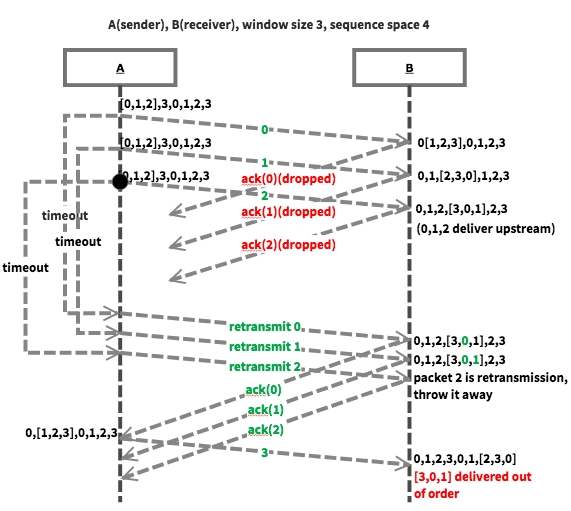
\includegraphics[height=.6\textheight]{./figures/9}
	\caption{Illustration of the Selective Repeat condition described in Problem 8}
\end{center}
\end{figure}
	

\end{document}